\documentclass[11pt,a4paper]{article}
\usepackage[utf8]{inputenc}
\usepackage[T1]{fontenc}
\usepackage{geometry}
\usepackage{graphicx}
\usepackage{booktabs}
\usepackage{caption}
\usepackage{array}
\usepackage{amsmath,amssymb,amsthm}
\usepackage[numbers]{natbib}
\usepackage{xurl}
\usepackage[colorlinks=true,linkcolor=blue,citecolor=blue,urlcolor=blue]{hyperref}
\usepackage{listings}

\geometry{
  left=2.5cm,
  right=2.5cm,
  top=2.5cm,
  bottom=2.5cm
}

\newcolumntype{L}[1]{>{\raggedright\arraybackslash}p{#1}}
\emergencystretch=2em

\title{\textbf{NRR-Patterns: Condition-Bounded Comparison of Five Delayed-Commitment Patterns in Stateful LLM Systems}}
\author{
  Kei Saito\thanks{ORCID: 0009-0006-4715-9176} \\
  Independent Researcher, Japan \\
  \texttt{kei.saito.research@gmail.com}
}
\date{April 2026 \\[0.5em]
\textit{Part of the Non-Resolution Reasoning (NRR) research program.}}

\begin{document}
\maketitle

\begin{center}
\textcopyright\ 2026 Kei Saito.
Licensed under CC BY 4.0.\\
\url{https://creativecommons.org/licenses/by/4.0/}
\end{center}

\begin{abstract}
Delayed-commitment recommendations in large language model systems are often
discussed too broadly or reused as if they transfer uniformly across providers
and task conditions. This paper compares five delayed-commitment patterns under
two matched \(t=0.0\) runs with live provider APIs, and then adds
provider-separated stability, temperature robustness, and selected Stage B
boundary checks to show where the comparison weakens, reverses, or becomes
non-effective. On the matched \(t=0.0\) comparison, Hierarchical Resolution,
Delta Update, Lazy Expansion, Conditional Refinement, and Branch Preservation
are all positive relative to their own paired baselines at the provider-
balanced aggregate level, while Branch remains only weakly positive. The
provider-separated view is less uniform: Branch already contains negative
Anthropic members before failing at Stage2, and Conditional weakens at Stage2
while retaining a positive provider-balanced aggregate despite an Anthropic-side
reversal. The Stage2 robustness result shows that Branch is the clearest
fragile case, but the failure shape is tail-risk-dominated rather than
provider-wide: the Gemini-side negative mean is driven mainly by one
catastrophic row, while the remaining Gemini rows are near-neutral in
aggregate. A compact compression comparison over a retained three-pattern
subset shows that the observed gains for that tested subset are not reducible
to generic prompt shortening: principle-only remains clearly positive within
each tested family-relative contrast, whereas compression-only weakens or fails
for key cases. Selected Stage B checks then show that a single aggregate
comparison view can hide provider-sensitive reversals and non-effective cells.
The result is a condition-bounded comparison whose main conclusions are kept
honest by explicit provider-separated stability, robustness, sign-flip, and
non-effective reporting rather than by a same-scale cross-family ranking or a
universal deployment rule.

\end{abstract}

\noindent\textbf{Keywords:} Non-Resolution Reasoning, delayed commitment, stateful LLM systems, paired comparison, provider-separated stability, boundary honesty

\section{Introduction}
\label{sec:intro}

Delayed commitment is useful in many stateful LLM workflows, but
recommendations built from that idea are easy to overgeneralize. A pattern
that reduces cost in one setting may weaken, reverse, or become non-effective
under another provider or operating condition. The main problem for this paper
is therefore not whether delayed commitment can ever help, but how to compare
five tested delayed-commitment patterns on one auditable matched-run design
while keeping the main comparison separate from the additional checks used to
expose sign-flip and non-effective regions. In this paper, the principal
comparison comes from the two matched \(t=0.0\) runs, while the selected Stage
B evidence serves as a separate boundary check rather than as part of the main
comparison itself.

Within the NRR series, fixed public lines establish first principles and
text-to-state mapping~\cite{saito2025nrr,saito2026phi}. Additional IME,
Transfer, and Coupled lines are cited for context rather than as direct
evidentiary supports for the claims made here~\cite{saito2026ime,saito2026transfer,saito2026coupled}. The role of this paper is narrower and more practical:
compare five delayed-commitment patterns under one matched paired design, then
report the resulting evidence through provider-separated stability,
temperature robustness, and selected Stage B boundary checks.

NRR is not an anti-LLM framework.
NRR does not replace standard LLM use.
NRR optimizes when to commit and when to defer, under explicit conditions.

\textbf{Series Consistency Statement:}
Across the NRR series, unsupported interpretations are not injected at a fixed evidence state, hypothesis-set expansion is evidence-gated, and unobserved possibilities remain explicitly unresolved. In NRR-Patterns, this policy is operationalized by keeping the main five-pattern comparison separate from additional boundary checks and by reporting unstable, sign-flip, and non-effective regions explicitly rather than hiding them behind winner-only summaries.

\textbf{Series Extensibility Statement:}
NRR should be read here as a derivation-and-evaluation framework, not as a closed recipe. The five delayed-commitment patterns in NRR-Patterns are an evaluated set under the present matched paired comparison plus explicit robustness and boundary checks, not an exhaustive set of admissible patterns. Additional patterns or operator-family extensions are in scope only when they are tested under the same paired-unit discipline and reported with equally explicit condition-bounded boundary language.

NRR-Patterns compares five delayed-commitment patterns under one matched paired
design and then adds provider-separated stability, temperature robustness, and
selected Stage B boundary checks to show where that map weakens, reverses, or
becomes non-effective.

The five canonical patterns are:
\begin{enumerate}
  \item Hierarchical Resolution
  \item Lazy Expansion
  \item Branch Preservation
  \item Delta Update
  \item Conditional Refinement
\end{enumerate}

These are treated here as delayed-commitment \emph{patterns}, not as the default meaning of lower-level \emph{operator} language used elsewhere in the series. That distinction matters because other papers in the series path also use \((\sigma/\delta,\text{target})\)-style operator language for interface-level update primitives, but those mentions are contextual here rather than evidentiary supports for the present pattern-comparison claims~\cite{saito2026phi,saito2026transfer,saito2026coupled}. The current paper instead evaluates pattern-level delayed-commitment designs.

\subsection{Contributions}

\begin{enumerate}
  \item A fixed matched-run comparison of five delayed-commitment patterns on two matched \(t=0.0\) runs.
  \item A separated provider-stability and temperature-robustness read showing where the comparison headline preserves, weakens, or breaks under provider-local condition shifts.
  \item A condition-bounded pattern map whose positive and unstable regions are supported by the matched comparison rather than by a same-scale cross-family ranking.
  \item Selected Stage B boundary checks for sign-flip and non-effective regions, showing where aggregate comparison reads can hide reversals or weak cells.
  \item A compression control over a retained three-pattern subset showing that those tested gains are not reducible to generic prompt shortening.
\end{enumerate}

\section{Related Work}
\label{sec:related}

\textbf{Delayed commitment and stateful interaction.}
Prior NRR work covers the failure mode and text-to-state mapping needed for stateful execution on stateless APIs in fixed public lines~\cite{saito2025nrr,saito2026phi}. Additional IME, Transfer, and Coupled references are retained here only to mark the broader series path and not as fixed evidentiary supports for the present comparison claims~\cite{saito2026ime,saito2026transfer,saito2026coupled}. The present paper does not reopen those layers. Instead, it compares multiple delayed-commitment patterns built on top of them and asks how that comparison should be read under explicit provider-sensitive boundaries.

\textbf{Efficiency and compression.}
Context-efficiency work, including retrieval compression and prompt-side compaction, targets token cost and context footprint directly~\cite{xu2023recomp,chevalier2023compress}. This paper overlaps in efficiency interest but differs in object: the main question is not simply whether prompts can be shortened, but whether delaying specific commitments yields a usable pattern map that remains condition-bounded once provider-sensitive boundary checks are surfaced. That is why the compression comparison is kept as a control rather than as the paper's main identity.

\textbf{Boundary-aware evaluation.}
Evaluation-framework work such as HELM, MT-Bench, and AlpacaEval shows that reported quality or preference conclusions can shift with benchmark protocol, judge setup, and reporting frame~\cite{liang2022helm,zheng2023mtbench,dubois2024alpacaeval}.

\textbf{Prompting and calibration sensitivity.}
Prompting and calibration work likewise shows that effect direction can change with reasoning prompts, aggregation strategy, and label-bias controls~\cite{kojima2022zeroshot,wang2023selfconsistency,zhao2021calibrate}. This manuscript adopts the shared lesson in a narrower form: it keeps one exact-replication paired spine, then reports a separated temperature-robustness member plus selected provider-sensitive boundary evidence so the comparison map is not over-read as a same-scale cross-family ranking.

\section{Pattern Set and Evaluation Logic}
\label{sec:method}

\subsection{Pattern Set and Paired Baselines}

Each pattern is evaluated under paired baseline-vs-pattern comparison with fixed scenario definitions and prompt templates inherited from the released comparison surfaces. Table~\ref{tab:pattern_catalog} states the pattern set, its baseline contrast, and the supported comparison/boundary profile under the current evidence.

\begin{table}[t]
\centering
\small
\begin{tabular}{L{3.0cm}L{4.2cm}L{2.5cm}L{4.0cm}}
\toprule
\textbf{Pattern} & \textbf{Paired baseline contrast} & \textbf{Delayed-commitment axis} & \textbf{Supported comparison/boundary profile} \\
\midrule
Hierarchical Resolution & flat full-option selection vs category-then-tool selection & decision granularity & positive family-relative benchmark with large within-family reduction \\
Lazy Expansion & eager full retrieval vs summary-first selective retrieval & content expansion & positive family-relative benchmark with later boundary sensitivity \\
Branch Preservation & no branch memory vs checkpointed branch restoration & branch destruction & provider-local instability case on the comparison surface \\
Delta Update & full-state resend vs changed-item-only updates & state retransmission & positive family-relative benchmark \\
Conditional Refinement & detailed-by-default vs coarse-first refinement & output detail & positive family-relative benchmark with sparse boundary support \\
\bottomrule
\end{tabular}
\caption{Canonical pattern catalog for NRR-Patterns. The table fixes the five compared patterns, their paired baseline contrasts, and the evidence profile used to interpret each family under the current comparison-plus-boundary read.}
\label{tab:pattern_catalog}
\end{table}

\subsection{Primary and Supporting Metrics}

The headline comparison metric is \emph{provider-balanced weighted reduction}
on the exact-replication comparison. The comparison contract for this quantity
is recorded in \path{repro/nrr_patterns_split_comparison_contract_v13_2026-04-12.md}.
For a given pattern and run, each provider first contributes its own weighted
reduction percentage, \(100 \times \sum_i (b_i - p_i) / \sum_i b_i\), over the
paired rows in that run's robust source file, where \(b_i\) and \(p_i\) denote
the baseline and pattern token totals for the same paired row. The run-level
quantity \path{weighted_percent_provider_balanced} is then the simple
arithmetic mean of those provider-level weighted percentages across providers.
Table~\ref{tab:comparison_summary} reports the two exact-replication run
values, their mean, and the separate Stage2 temperature-robustness result,
while Table~\ref{tab:provider_separated_stability} reports the compact
provider-separated stability summary derived from the same paired rows.
Supporting comparison metrics remain weighted global reduction, median
reduction, trimmed reduction, and cost-per-success delta.

\subsection{Boundary-Honesty Metrics}

The selected boundary metrics are misinterpretation improvement and rework
improvement. Here ``Stage B'' means the historical all-pattern confirmatory
boundary-resolution suite in the `nrr-boundary' package, from which this paper
uses only a small subset. The selection rule is recorded in
\path{repro/nrr_patterns_stageb_selection_rule_v2_2026-04-12.md}. The
retained pair is the smallest downstream quality/cost pair that can keep the
five-pattern comparison honest without turning NRR-Patterns into a second
boundary-focused paper. Additional diagnostics such as trace completeness,
update consistency, internal coherence error rate, self-contradiction rate,
and selected stability diagnostics remain available as secondary surfaces when
they materially sharpen the interpretation.

\subsection{Reporting Rules and Validity Limits}

Use provider-balanced results for the headline comparison and provider-separated results for boundary honesty where aggregation could hide reversals.

The canonical result-language ladder is:
\begin{itemize}
  \item positive region
  \item unstable region
  \item sign-flip region
  \item non-effective region
\end{itemize}

The main comparison surface primarily supports the positive/unstable read. Sign-flip and non-effective labels are carried by selected boundary checks where those regions are directly observed. Accordingly, these labels should not be misread as if they were all outputs of the headline comparison metric alone.

\section{Experimental Surfaces}
\label{sec:surfaces}

\subsection{Main Comparison Surface}

The primary experimental surface uses the exact-replication five-pattern
comparison in the released NRR-Patterns materials. Here, exact replication
means the fixed auditable matched-run outputs named below, not a rerun-capable
environment. The
provider/model scope is Anthropic Claude Sonnet 4
(\texttt{claude-sonnet-4-20250514}), Gemini 2.0 Flash
(\texttt{gemini-2.0-flash}), and OpenAI GPT-4o mini
(\texttt{gpt-4o-mini-2024-07-18}):
\begin{itemize}
  \item Stage1 main (\(t=0.0\))
  \item Stage1 rep2 (\(t=0.0\))
\end{itemize}

These two \(t=0.0\) runs define the main exact-replication comparison. The
comparison names are recorded in
\path{repro/nrr_patterns_comparison_claims_manifest_v7_2026-04-12.csv}, and
the fairness/aggregation contract for separating exact replication from
robustness is recorded in
\path{repro/nrr_patterns_split_comparison_contract_v13_2026-04-12.md}. The
comparison headline summary is
\path{results/analysis/nrr_patterns_comparison_headline_summary_v3_2026-04-12.csv},
the compact provider-separated stability summary is
\path{results/analysis/nrr_patterns_provider_separated_stability_summary_v3_2026-04-12.csv},
and the headline source members are:
\begin{itemize}
  \item \path{results/nrr_patterns_results_allproviders_clean.zip::results/analysis/nrr_patterns_allproviders_pattern_summary_robust_t00.csv}
  \item \path{results/nrr_patterns_results_stage1_t00_rep2.zip::results/analysis/nrr_patterns_allproviders_pattern_summary_robust_t00.csv}
\end{itemize}
The separate temperature-robustness result is:
\begin{itemize}
  \item \path{results/nrr_patterns_results_stage2_t03.zip::results/analysis/nrr_patterns_allproviders_pattern_summary_robust_t03.csv}
\end{itemize}
The paper therefore reports one exact-replication summary while keeping the
robustness result separate rather than collapsing all three members into one
undifferentiated mean.

\subsection{Compression Comparison}

The compression comparison remains in the main manuscript as a compact
interpretive control. Its role is to test whether the observed gains can be
explained by generic prompt compression rather than by delayed commitment
itself. The comparison is recorded in
\path{repro/nrr_patterns_comparison_claims_manifest_v7_2026-04-12.csv}. The
aggregated control surface is
\path{results/analysis/nrr_patterns_comparison_summary_r2_aggregated.csv},
with per-provider drill-down in
\path{results/analysis/nrr_patterns_comparison_summary_r2_by_provider.csv}
and raw comparison traces inside the three provider ZIP artifacts.

\subsection{Selected Stage B Boundary-Resolution Surface}

Selected Stage B evidence enters this paper as a boundary-check layer, not as
the paper's primary confirmatory center. Here, ``Stage B'' refers to the
historical `nrr-boundary' confirmatory boundary-resolution suite over the same
five delayed-commitment families, but this paper uses only the selected subset
named here. The relevant file names are recorded in
\path{repro/nrr_patterns_boundary_claims_manifest_v2_2026-04-12.csv}, and the
selection rule is recorded in
\path{repro/nrr_patterns_stageb_selection_rule_v2_2026-04-12.md}. The
retained pair \texttt{misinterpretation\_rate} plus
\texttt{rework\_cost\_tokens} is the smallest downstream quality/cost pair
needed to keep the comparison honest. In this package, the selected
Stage B evidence is traceable to:
\begin{itemize}
  \item \path{nrr-boundary/stats/stageb_all/mst_provider_balanced.csv}
  \item \path{nrr-boundary/stats/stageb_all/mst_provider_separated.csv}
  \item \path{nrr-boundary/stats/stageb_all/mst_sign_flip_boundaries.csv}
  \item \path{nrr-boundary/stats/stageb_all/stageb_confirmatory_tests_holm30.csv}
\end{itemize}
These files are used only to show where the comparison map weakens, reverses,
or becomes non-effective. They do not replace the token-efficiency headline,
and they do not turn this paper into a second boundary-focused manuscript.

\subsection{Secondary Appendix Materials}

Ordered-combination follow-up, rep1-vs-rep3 direction details, and no-position
ablation are not part of the default main-text claim hierarchy. Ordered composition remains
secondary because it introduces a separate provider-by-order interaction story
that can easily dominate the paper if over-promoted. The no-position ablation
remains useful as a robustness check, but it is not required for the main
comparison claim hierarchy. Both therefore
remain in the appendix by default.

\section{Results: Pattern Comparison}
\label{sec:results_comparison}

\subsection{Provider-Balanced Pattern Map}

Across the two exact-replication comparison runs, provider-balanced weighted
reduction remains strongly heterogeneous rather than uniform.
Table~\ref{tab:comparison_summary} gives the current summary from the
comparison headline summary named in Sec.~\ref{sec:surfaces}, while keeping the
Stage2 temperature-robustness member separate from the headline mean.
\begin{table}[t]
\centering
\small
\begin{tabular}{L{2.2cm}L{1.3cm}rrrr}
\toprule
\textbf{Pattern} & \textbf{Rows} & \textbf{S1 main} & \textbf{S1 rep2} & \textbf{Rep. mean} & \textbf{S2} \\
\midrule
Hierarchical & 45 & \(+56.752\%\) & \(+57.606\%\) & \(+57.179\%\) & \(+55.737\%\) \\
Delta & 18 & \(+39.074\%\) & \(+38.956\%\) & \(+39.015\%\) & \(+38.980\%\) \\
Lazy & 45 & \(+37.951\%\) & \(+37.459\%\) & \(+37.705\%\) & \(+38.066\%\) \\
Conditional & 18 & \(+37.011\%\) & \(+35.353\%\) & \(+36.182\%\) & \(+32.235\%\) \\
Branch & 45 & \(+2.452\%\) & \(+3.081\%\) & \(+2.766\%\) & \(-21.713\%\) \\
\bottomrule
\end{tabular}
\caption{Provider-balanced weighted reduction under the split comparison contract. The headline mean uses only the two exact-replication \(t=0.0\) runs, while Stage2 \((t=0.3)\) is reported separately as the robustness member. The surface is not evidence-symmetric across patterns: Hierarchical, Lazy, and Branch carry \(n_{\mathrm{all}}=45\) paired rows per run, whereas Delta and Conditional carry \(n_{\mathrm{all}}=18\). The magnitudes are not directly comparable across families as a same-scale ranking because each family uses its own paired baseline contrast and token-cost floor.}
\label{tab:comparison_summary}
\end{table}

The resulting exact-replication read should therefore be interpreted with explicit paired-row-volume asymmetry, non-comparable family baseline contrasts, and provider-separated stability in view:
\begin{itemize}
  \item Hierarchical, Delta, and Lazy remain positive for Anthropic, Gemini, and OpenAI across the two exact-replication runs and the separated robustness member.
  \item Conditional is positive for all three providers on exact replication, but the Stage2 robustness member contains an Anthropic-side reversal even though the provider-balanced aggregate stays positive.
  \item Branch is aggregate-positive on exact replication but already contains negative Anthropic exact-replication members, then fails the separated robustness member through a Gemini-led, tail-risk-dominated collapse.
\end{itemize}

\subsection{Replication and Temperature Robustness}

NRR-Patterns retains the Stage2 member because the main issue is not just exact replication but also whether the same paired comparison object survives a controlled condition shift. That robustness member must be read separately rather than folded into the headline mean. Hierarchical, Delta, and Lazy remain positive for all three providers in both exact-replication runs and in Stage2. Conditional, by contrast, weakens at \(t=0.3\) and flips negative on Anthropic even though the provider-balanced Stage2 aggregate remains positive. Branch is the clearest failure case: it is slightly aggregate-positive in both \(t=0.0\) runs despite negative Anthropic exact-replication members, then turns sharply negative in Stage2 because Gemini contains a tail-risk event that pulls down the provider-balanced aggregate rather than producing a uniform all-provider collapse. That is why the NRR-Patterns reads Branch as a fragile provider-local case rather than as a robust fifth positive family benchmark.

\begin{figure}[t]
\centering
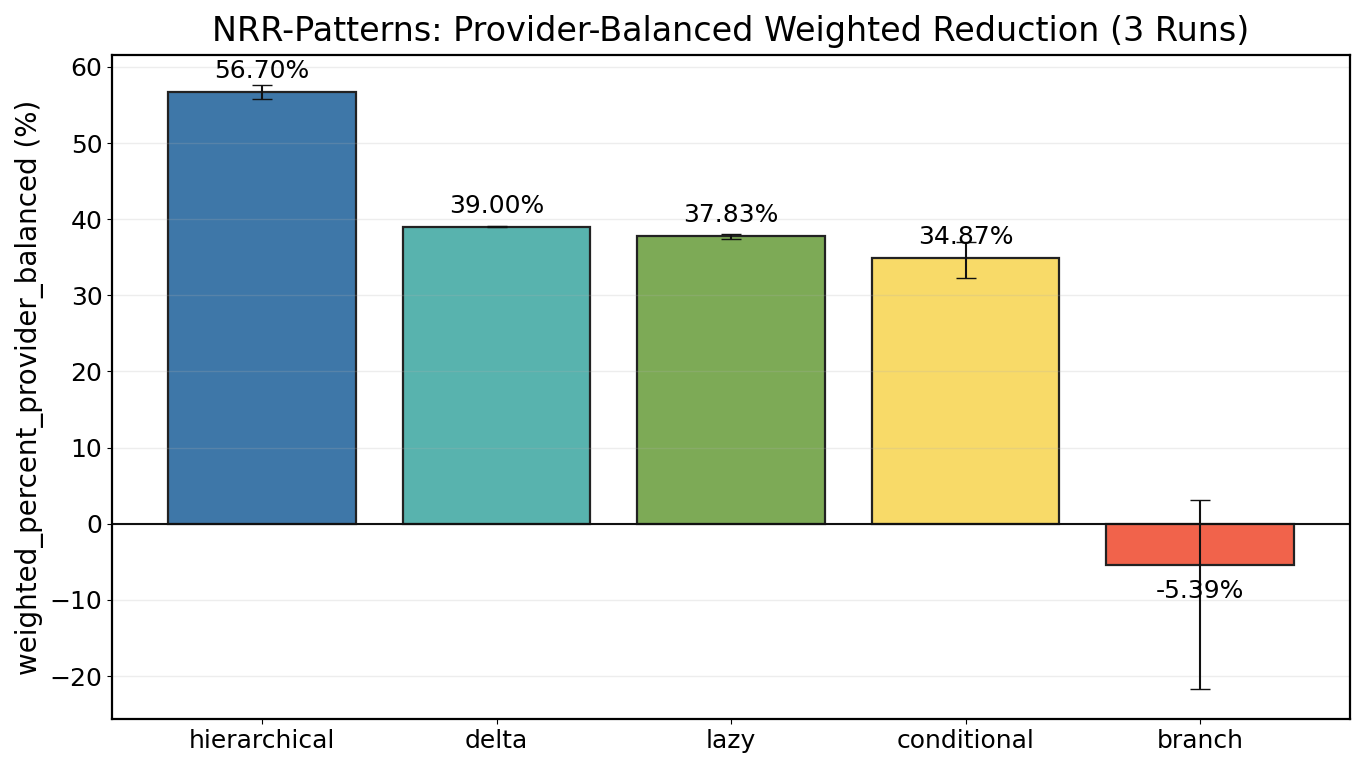
\includegraphics[width=0.92\textwidth]{../figures/fig_patterns_weighted_3runs.png}
\caption{Provider-balanced weighted reduction across the two exact-replication runs plus the separated Stage2 robustness member. Error bars show the observed range over these members for each pattern. The plotted magnitudes remain family-relative against different paired baselines and should not be read as a same-scale cross-family ranking.}
\label{fig:nrr_patterns_comparison_3runs}
\end{figure}

\subsection{Provider-Separated Stability Read}

The split comparison surface already shows that exact-replication positivity is not the same as universal safety. Table~\ref{tab:provider_separated_stability} makes that point visible inside the main text rather than leaving it only in the shipped ZIP members. Branch is the clearest example: it stays slightly aggregate-positive on the exact-replication spine, but Anthropic is already negative in both exact-replication runs, and the Stage2 negative turn is driven by Gemini rather than by uniform all-provider collapse. Conditional is less severe but still illustrates the same principle by weakening materially at \(t=0.3\) while carrying an Anthropic-side reversal inside an aggregate-positive provider-balanced read. The other three patterns are substantially more stable across the split comparison read, but even there the correct interpretation is still condition-bounded rather than universal. This is why NRR-Patterns stops at a comparison-led family benchmark map and then carries boundary honesty separately, rather than converting the comparison table into a deployment-wide ranking.

\begin{table}[t]
\centering
\small
\begin{tabular}{L{1.85cm}L{2.7cm}L{2.7cm}L{2.7cm}L{3.75cm}}
\toprule
\textbf{Pattern} & \textbf{S1 main (A/G/O)} & \textbf{S1 rep2 (A/G/O)} & \textbf{S2 (A/G/O)} & \textbf{Comparison-side read} \\
\midrule
Hierarchical & A +41.3 / G +71.0 / O +57.9 & A +41.3 / G +74.2 / O +57.3 & A +41.7 / G +68.2 / O +57.4 & all-provider positive across the exact-replication spine and the separated robustness member \\
Delta & A +33.1 / G +35.9 / O +48.2 & A +33.7 / G +34.6 / O +48.6 & A +32.5 / G +38.9 / O +45.6 & all-provider positive across the comparison surface, but with lower support volume than Hierarchical/Lazy/Branch \\
Lazy & A +47.6 / G +41.1 / O +25.1 & A +47.6 / G +40.7 / O +24.1 & A +47.9 / G +42.1 / O +24.2 & all-provider positive on comparison and robustness, with later degradation appearing in the boundary layer \\
Conditional & A +6.8 / G +64.1 / O +40.1 & A +6.3 / G +61.0 / O +38.8 & A -4.1 / G +58.0 / O +42.8 & exact-replication all-provider positive, but Stage2 contains an Anthropic-side reversal inside an aggregate-positive read \\
Branch & A -0.1 / G +6.2 / O +1.2 & A -1.1 / G +6.4 / O +4.0 & A +5.3 / G -74.3 / O +3.9 & aggregate-positive exact replication with Anthropic instability, then Gemini-led Stage2 failure \\
\bottomrule
\end{tabular}
\caption{Compact provider-separated weighted reduction summary, derived from
the provider-separated stability summary artifact in the shipped audit files.
Provider order is Anthropic/Gemini/OpenAI. This table makes the comparison-side
instability visible in the main text instead of leaving it only inside the
shipped paired-delta ZIP members.}
\label{tab:provider_separated_stability}
\end{table}

The Branch failure shape is also narrower than a broad provider-wide collapse. In the Stage2 Gemini paired-delta member \path{results/nrr_patterns_results_stage2_t03.zip::results/analysis/nrr_patterns_prod_gemini_clean_t03_paired_deltas.csv}, the worst Branch row is \texttt{scenario3 / repetition3}, where the token count changes from \texttt{3372} to \texttt{38998} (\(-1056.524318\%\)). The Gemini Branch provider-weighted Stage2 value is \(-74.326453\%\) with that row included, but the compact provider-separated summary also records that it would be only \(-0.530303\%\) without that one worst row. The appropriate reading is therefore tail-risk-dominated robustness failure, not a broad all-row or all-provider collapse.

\subsection{Pattern Status Ladder}

The end of the comparison section summarizes the main read in one compact
status ladder. Table~\ref{tab:status_ladder} states the current NRR-Patterns
summary.

\begin{table}[t]
\centering
\small
\begin{tabular}{L{2.2cm}L{1.2cm}L{2.6cm}L{5.5cm}}
\toprule
\textbf{Pattern} & \textbf{Rows} & \textbf{Split status} & \textbf{Boundary note} \\
\midrule
Hierarchical & 45 & robust positive region & remains strong on the exact-replication spine, but later boundary views still matter for provider-sensitive weakening cells \\
Lazy & 45 & robust positive region & exact-replication positive and robustness-positive, but carried-forward boundary views expose weaker and degrading cells \\
Branch & 45 & aggregate-positive instability / tail-risk robustness failure & exact replication is only aggregate-positive because Anthropic is already negative, and the separated robustness member fails through a Gemini-led tail-risk event \\
Delta & 18 & robust positive region & exact-replication positive and robustness-positive, but selected boundary checks expose weaker cells \\
Conditional & 18 & aggregate-positive with Stage2 provider reversal & clearest positive provider-mean support on the retained key metrics, but Stage2 already contains an Anthropic-side comparison reversal and the boundary layer stays sparse/non-uniform \\
\bottomrule
\end{tabular}
\caption{NRR-Patterns status ladder under the split comparison contract. Status is assigned from the exact-replication spine plus the separated robustness member, while the rows/run column exposes the unequal paired-row counts behind the five-pattern map. Unequal paired-row volume is not equivalent to unequal independent support thickness.}
\label{tab:status_ladder}
\end{table}

\section{Results: Boundary and Control Checks}
\label{sec:results_boundary}

\subsection{Compression Is Not a Drop-In Substitute}

The compression control stays in the main text because it answers the most natural skepticism against a comparison-led delayed-commitment paper: perhaps the gains come only from shorter prompts. The current aggregated comparison, however, does not support that simpler story for the retained three-pattern subset. Table~\ref{tab:r2_takeaway_nrr_patterns} shows that principle-only remains clearly positive for all three tested patterns, whereas compression-only is negative for Hierarchical and Delta and only near-neutral for Lazy.

\begin{table}[t]
\centering
\small
\begin{tabular}{lrrr}
\toprule
\textbf{Pattern} & \textbf{Principle-only} & \textbf{Compression-only} & \textbf{Principle+compression} \\
\midrule
Delta & \(+38.148\%\) & \(-25.623\%\) & \(+3.324\%\) \\
Hierarchical & \(+57.212\%\) & \(-8.224\%\) & \(+36.675\%\) \\
Lazy & \(+38.207\%\) & \(+1.523\%\) & \(+8.589\%\) \\
\bottomrule
\end{tabular}
\caption{Provider-balanced weighted reduction for the retained r2 compression comparison. Values are read from the aggregated r2 comparison summary artifact described in Sec.~\ref{sec:surfaces}.}
\label{tab:r2_takeaway_nrr_patterns}
\end{table}

The comparative structure matters. Principle-only remains the strongest read for all three tested patterns, while the combination condition stays positive but weaker than principle-only. The provider-separated control rows also show why this section must remain condition-bounded rather than aggregate-only: for Hierarchical, compression-only is negative on Anthropic and OpenAI but positive on Gemini, while for Lazy it is positive on Anthropic and OpenAI but strongly negative on Gemini. Compression-only therefore functions as a useful control for this retained subset, but not as an equivalent or provider-invariant substitute for delayed-commitment patterning on that tested three-pattern slice.

\begin{figure}[t]
\centering
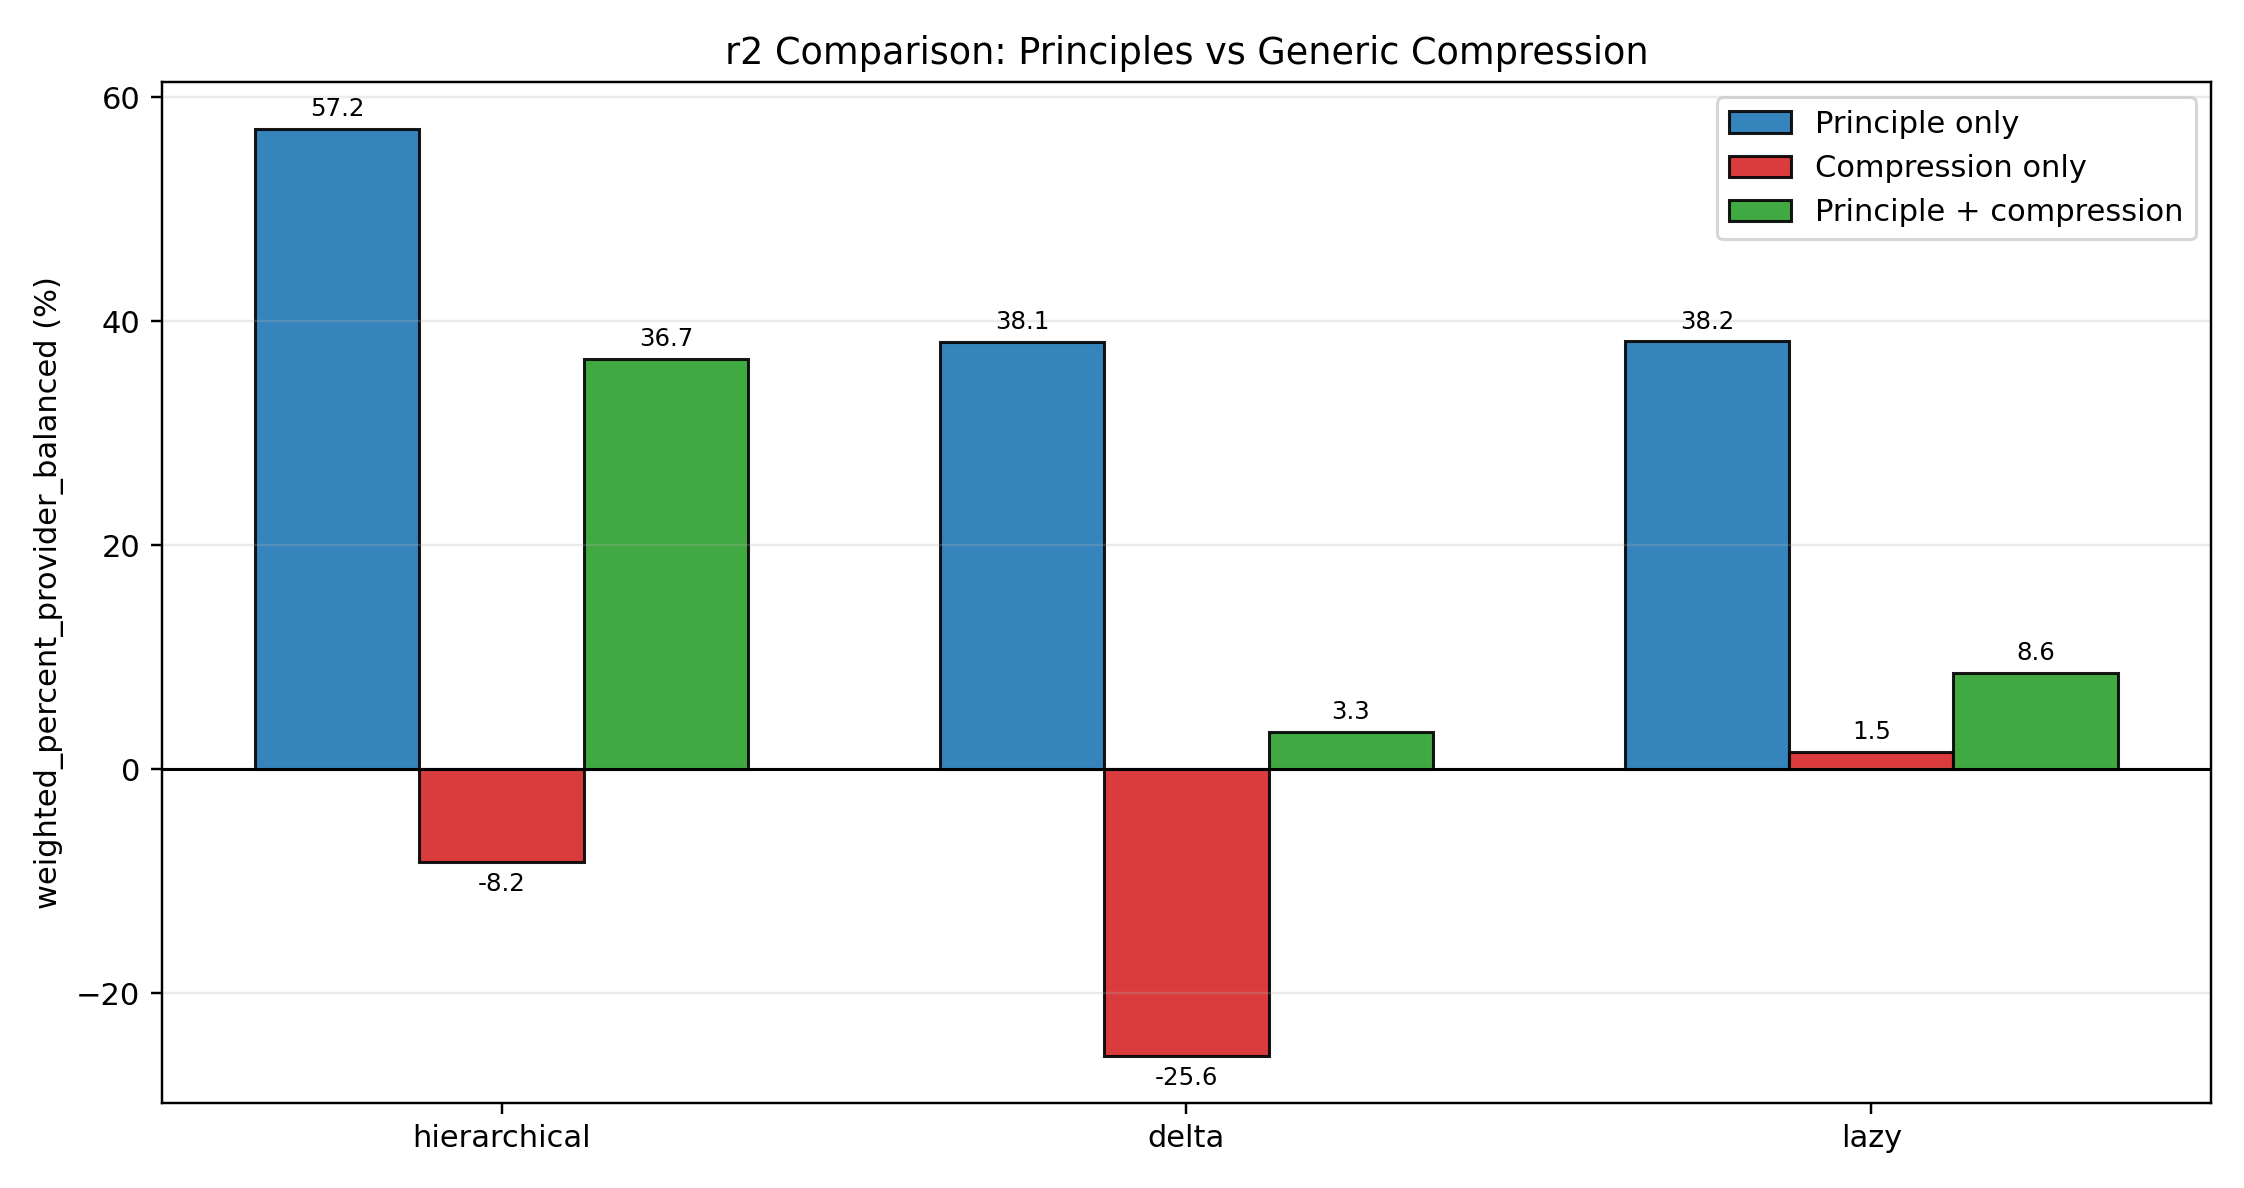
\includegraphics[width=0.95\textwidth]{../figures/fig_r2_comparison_weighted.png}
\caption{Compression control for the retained three-pattern subset. Principle-only remains strongest, while compression-only weakens or fails for key cases.}
\label{fig:nrr_patterns_r2_comparison}
\end{figure}

\subsection{Selected Stage B Boundary Checks}

Selected Stage B evidence is included only to show where provider-separated
quality behavior weakens, reverses, or becomes non-effective. This Stage B
layer is a selected subset of the historical `nrr-boundary' confirmatory
suite, not a new manuscript-native experiment block. The retained
\texttt{misinterpretation\_rate} plus \texttt{rework\_cost\_tokens} pair is
the smallest downstream quality/cost pair needed for honest reporting.
Table~\ref{tab:stageb_selected_nrr_patterns} summarizes the two key metrics
retained for this role.

\begin{table}[t]
\centering
\small
\begin{tabular}{lrr}
\toprule
\textbf{Pattern} & \textbf{Misinterpretation improvement} & \textbf{Rework improvement (tokens)} \\
\midrule
Conditional & \(+0.0781\) & \(+122.6481\) \\
Hierarchical & \(+0.0120\) & \(-12.1852\) \\
Delta & \(+0.0028\) & \(-26.6296\) \\
Branch & \(-0.0006\) & \(-24.7222\) \\
Lazy & \(-0.1242\) & \(-234.3704\) \\
\bottomrule
\end{tabular}
\caption{Selected Stage B provider-balanced key-metric improvements, read from the Stage B provider-balanced artifact described in Sec.~\ref{sec:surfaces}. Positive values indicate improvement over baseline.}
\label{tab:stageb_selected_nrr_patterns}
\end{table}

These boundary checks change how the comparison map should be read:
\begin{itemize}
  \item Conditional has the clearest positive provider-mean support on the retained Stage B key metrics, but that support remains sparse rather than uniformly active.
  \item Lazy is the clearest degraded pattern on the retained confirmatory surface, with negative provider-balanced means on both retained key metrics.
  \item Hierarchical, Delta, and Branch show provider-sensitive weakening or reversal cells rather than a clean all-provider positive read.
  \item Sign-flip and non-effective regions must be reported explicitly rather than hidden behind pooled summaries.
\end{itemize}

The provider-separated read makes the same point more sharply. Conditional
remains positive on provider means for misinterpretation and rework across
Anthropic, OpenAI, and Gemini, but the support is still sparse rather than
uniformly active: in
\path{nrr-boundary/stats/stageb_all/stageb_confirmatory_tests_holm30.csv},
misinterpretation carries \(n_{\mathrm{nonzero}}=25/54\) and rework carries
\(33/54\), and the provider-separated rows still contain substantial zero-count
mass plus some negative rework cases. By contrast, Hierarchical flips negative
on Gemini for both retained key metrics, Delta is negative on Anthropic and
Gemini for rework, Branch is negative on Gemini for both retained key metrics,
and Lazy is strongly negative on Gemini while only weakly positive or
near-neutral elsewhere. On the comparison surface, this same provider-local
structure is why Branch should be read as a localized instability case rather
than as a uniformly collapsing family. Stage B therefore functions as a
boundary-check layer rather than as a replacement for the main comparison.

Sign-flip evidence is also direct rather than rhetorical. In the current Stage B boundary artifact, sign-flip boundaries appear in 20 of 45 pattern-metric cells. Conditional shows no Stage B sign-flip cells under this setup, while Branch, Delta, Hierarchical, and Lazy all show sign-flip boundaries on multiple metrics. Figure~\ref{fig:nrr_patterns_stageb_signflip} is included here for compact honesty reporting rather than for boundary-paper completeness.

\begin{figure}[t]
\centering
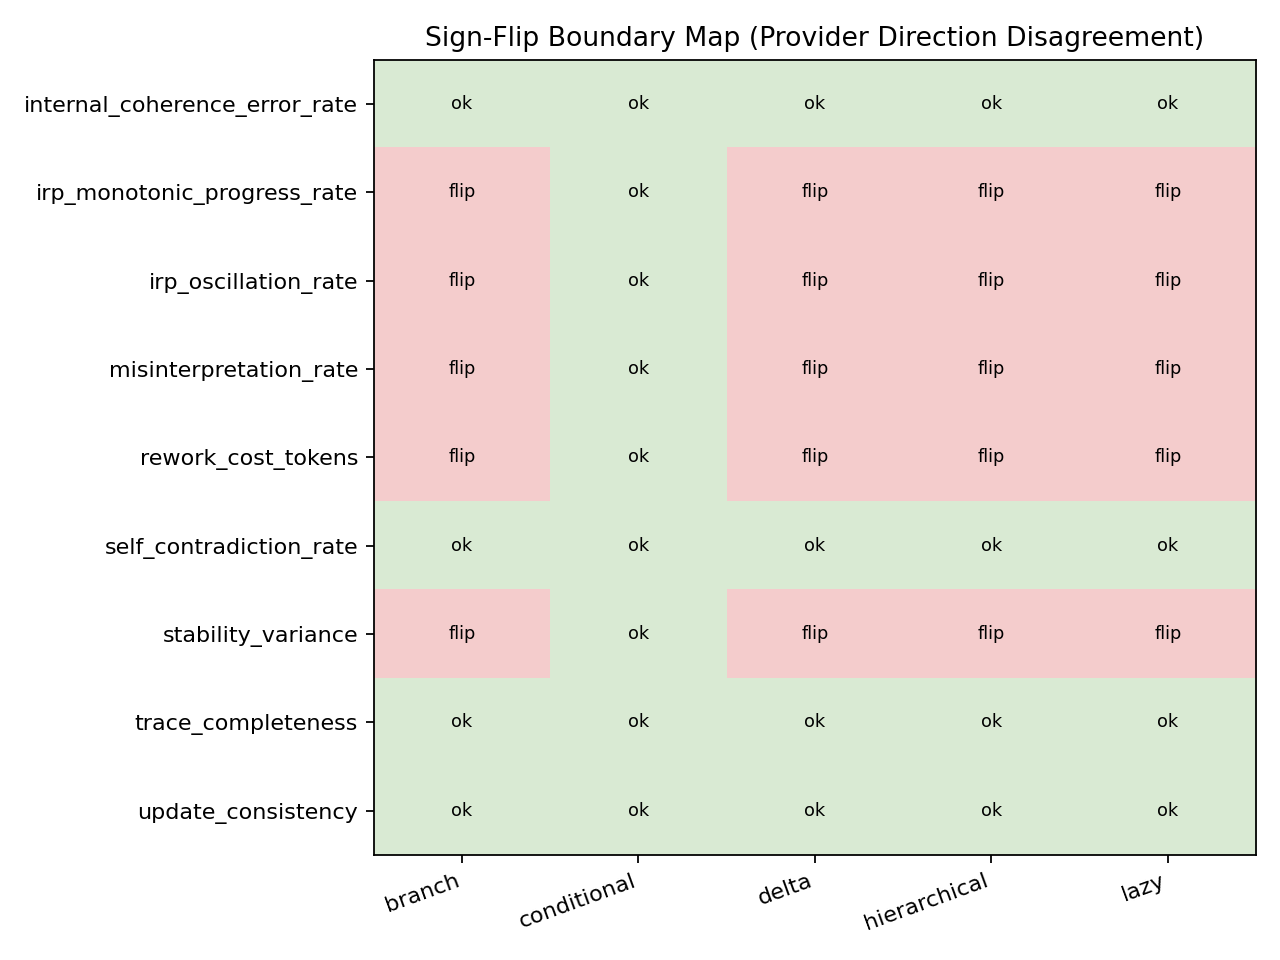
\includegraphics[width=0.95\textwidth]{../figures/nrr_patterns_stageb_sign_flip_boundaries.png}
\caption{Selected Stage B sign-flip boundary map carried forward as the honesty layer for NRR-Patterns.}
\label{fig:nrr_patterns_stageb_signflip}
\end{figure}

The confirmatory results are consistent with this reading. In
\path{nrr-boundary/stats/stageb_all/stageb_confirmatory_tests_holm30.csv},
only five Holm-significant cells survive correction: two positive cells for
Conditional (misinterpretation and rework) and three degraded cells for Lazy
(update consistency, internal coherence, and self-contradiction). This is
enough to keep the positive comparison story honest, but not enough to turn the
paper into a second confirmatory study of operator boundaries.

Non-effective reporting is also part of the paper rather than a
supplement-only afterthought. Table~\ref{tab:stageb_noneffective_nrr_patterns}
lists the selected Stage B metrics whose provider-separated artifact shows
all-provider zero cells under the current setup. These cells do not overturn
the main comparison read by themselves, but they do mark regions where a
positive interpretation should stop short of claiming an active effect.

\begin{table}[t]
\centering
\small
\begin{tabular}{L{2.4cm}L{8.8cm}}
\toprule
\textbf{Pattern} & \textbf{All-provider zero metrics on selected Stage B} \\
\midrule
Conditional & internal coherence error rate; trace completeness \\
Delta & internal coherence error rate; trace completeness \\
Branch & internal coherence error rate; trace completeness \\
Hierarchical & none in the selected all-provider-zero slice \\
Lazy & none in the selected all-provider-zero slice \\
\bottomrule
\end{tabular}
\caption{Selected Stage B all-provider non-effective cells. A cell appears here when the provider-separated honesty artifact reports zero-direction behavior for Anthropic, Gemini, and OpenAI under the current setup. Provider-specific zero or near-zero cells remain in the shipped provider-separated artifact even when they do not rise to the all-provider slice shown here.}
\label{tab:stageb_noneffective_nrr_patterns}
\end{table}

\section{Discussion}
\label{sec:discussion}

\subsection{What the Pattern Map Supports}

The supported read is condition-bounded utility, not universal superiority. On
the exact-replication comparison, all five patterns are aggregate-positive
relative to their own paired baselines, but they do not remain equally strong
once the provider-separated stability table, the robustness result, and the
boundary evidence are added. Hierarchical and Delta remain robustly positive on
the split comparison surface. Lazy remains positive on the exact-replication
comparison and the robustness result, but its boundary read is degraded rather
than robustly positive. Conditional stays aggregate-positive but already
contains a Stage2 provider-side reversal. Branch fails even earlier by showing
exact-replication Anthropic instability and then losing positive status on the
robustness result through a tail-risk-dominated provider-local failure. The
appropriate output is therefore a family-benchmark pattern map, not a same-
scale ranking.

\subsection{Why Provider Sensitivity Changes the Read}

Provider-balanced summaries are useful for the exact-replication headline, but
the robustness result and provider-separated views are necessary where
aggregation can hide reversals or tail-risk concentration. This paper
therefore distinguishes four evidence roles: exact replication for the main
family-benchmark read, provider-separated stability for comparison-side
reversals and concentration, robustness for controlled condition-shift stress,
and boundary checks for the caveat layer. Collapsing those roles would either
overstate the comparison or overinflate the boundary section.

\subsection{Why Compression Is Not Enough}

The compact control against generic prompt compression matters because it distinguishes delayed-commitment patterning from a simpler prompt shortening story. On the retained r2 surface, principle-only stays clearly positive where compression-only weakens or fails for the three tested patterns. This does not prove that compression is never useful; it shows that the tested subset gains are not adequately explained by prompt shortening alone.

\subsection{How to Read Unstable, Sign-Flip, and Non-Effective Regions}

These regions are not embarrassing leftovers. They are part of the contribution because they define where reuse becomes unsafe, unsupported, or too weak to generalize under the current evidence state. In this paper, unstable is primarily a comparison-side label, while sign-flip and non-effective are boundary-honesty labels. Keeping those roles distinct is part of the manuscript's scientific honesty.

\subsection{Series Position}

NRR-Patterns is the pattern-comparison layer upstream of Energy. It is not the
calibration paper, and it is not the downstream closure paper. Its job is to
make the comparison evidence clear enough that later calibration and closure
work do not inherit a blurred pattern story.

\section{Limitations}
\label{sec:limitations}

This paper cites traceable comparison and Stage B values directly from the
released analysis files, and the naming conventions are recorded in the
manifests. The released artifact set is auditable rather than a full rerun
bundle: it includes the manuscript assets, the comparison and boundary
manifests, a checksum manifest, and the named comparison and boundary files
needed for inspection. Here, exact replication means that the fixed matched-run
outputs can be audited and examined from preserved summaries and run-specific
members; it does not mean that the distributed bundle is itself a full
independent rerun environment. Provider sensitivity remains real and must not
be hidden by a single aggregate summary, and the five-pattern map is based on
unequal paired-row volume across patterns. That paired-row volume is useful for
auditability, but it is not the same thing as independent support thickness.
Ordered composition remains outside the main-text claim hierarchy, and
no-position ablation remains appendix-first rather than main-text essential.

\section{Conclusion}
\label{sec:conclusion}

NRR-Patterns supports a condition-bounded pattern map over five delayed-
commitment patterns under a split comparison contract. On the exact-replication
comparison, all five patterns remain aggregate-positive relative to their own
paired baselines, but the provider-separated stability summary and the
temperature-robustness result show that those positives are not equally stable.
Hierarchical and Delta remain robustly positive on the split comparison
surface, Lazy stays positive on comparison and robustness while degrading in
the boundary checks, Conditional remains aggregate-positive but already
contains a Stage2 provider-side reversal, and Branch becomes the clearest
fragile provider-local case because exact-replication Anthropic instability is
followed by a Gemini-led, tail-risk-dominated Stage2 failure rather than by
uniform collapse across providers. A compact compression control over the
retained three-pattern subset shows that those tested gains are not reducible
to generic prompt shortening alone. The supported output is therefore not a
universal ranking, but a comparison-led family benchmark map with explicit
provider-separated stability, robustness, sign-flip, and non-effective
regions.

\section{Reproducibility and Appendix Home}
\label{sec:repro}

The current NRR-Patterns release is organized as an auditable evidence package
rather than a full end-to-end rerun bundle. The package map is recorded in
\path{repro/nrr_patterns_package_map_v20_2026-04-12.md}, the split comparison contract is recorded in
\path{repro/nrr_patterns_split_comparison_contract_v13_2026-04-12.md}, the
Stage B selection rule is recorded in
\path{repro/nrr_patterns_stageb_selection_rule_v2_2026-04-12.md}, the
release-manifest checksum anchor is
\path{repro/nrr_patterns_repro_checksums_sha256.txt}, and the shipped audit
checksum manifest is
\path{repro/nrr_patterns_audit_surface_sha256_v20_2026-04-12.txt}. The main
comparison files are:
\begin{itemize}
  \item \path{results/analysis/nrr_patterns_comparison_headline_summary_v3_2026-04-12.csv}
  \item \path{results/analysis/nrr_patterns_provider_separated_stability_summary_v3_2026-04-12.csv}
  \item \path{results/nrr_patterns_results_allproviders_clean.zip::results/analysis/nrr_patterns_allproviders_pattern_summary_robust_t00.csv}
  \item \path{results/nrr_patterns_results_allproviders_clean.zip::results/analysis/nrr_patterns_allproviders_paired_deltas_merged_t00.csv}
  \item \path{results/nrr_patterns_results_stage1_t00_rep2.zip::results/analysis/nrr_patterns_allproviders_pattern_summary_robust_t00.csv}
  \item \path{results/nrr_patterns_results_stage2_t03.zip::results/analysis/nrr_patterns_allproviders_pattern_summary_robust_t03.csv}
  \item \path{results/nrr_patterns_results_stage2_t03.zip::results/analysis/nrr_patterns_allproviders_paired_deltas_merged_t03.csv}
  \item \path{results/nrr_patterns_results_stage2_t03.zip::results/analysis/nrr_patterns_prod_gemini_clean_t03_paired_deltas.csv}
  \item \path{results/analysis/nrr_patterns_comparison_summary_r2_aggregated.csv}
\end{itemize}

The selected boundary-check files are:
\begin{itemize}
  \item \path{nrr-boundary/stats/stageb_all/mst_provider_balanced.csv}
  \item \path{nrr-boundary/stats/stageb_all/mst_provider_separated.csv}
  \item \path{nrr-boundary/stats/stageb_all/mst_sign_flip_boundaries.csv}
  \item \path{nrr-boundary/stats/stageb_all/stageb_confirmatory_tests_holm30.csv}
\end{itemize}

Appendix materials include the no-position ablation
(\path{results/nrr_patterns_no_position_t00.zip}, \path{results/analysis/nrr_patterns_no_position_summary.csv}).
An ordered-combination follow-up is also retained outside the main-text claim
hierarchy, but it is named for traceability only and is omitted from the
current default audit bundle. Only the no-position ablation is shipped in the
current audit bundle.

The current NRR-Patterns checksum manifest is
\path{manuscript/checksums_active_review_surface_sha256.txt}. In the current
release, \path{scripts/verify_current_package.sh} verifies the manuscript asset
set together with the release manifests, while
\path{scripts/verify_audit_surface.py} verifies the listed audit files
against the audit checksum manifest. Together, the package map, the split
comparison contract, the Stage B selection rule, the comparison summaries, the
release-manifest checksum anchor, the audit checksum manifest, and the current
manuscript checksum manifest define the documented artifact set for this paper.

\section*{Acknowledgments}
The author acknowledges the use of large language models, including Claude
(Anthropic), ChatGPT/Codex (OpenAI), and Gemini (Google), for language
editing, proofreading, and LaTeX formatting assistance during manuscript
preparation. All substantive ideas, claims, analyses, and conclusions are
solely the responsibility of the author.

\begin{thebibliography}{99}\sloppy

\bibitem{saito2025nrr}
Saito, K. (2025).
\textit{NRR-Core: Non-Resolution Reasoning as a Computational Framework for Contextual Identity and Ambiguity Preservation}.
arXiv:2512.13478.

\bibitem{saito2026phi}
Saito, K. (2026).
\textit{NRR-Phi: Text-to-State Mapping for Ambiguity Preservation in LLM Inference}.
arXiv:2601.19933.

\bibitem{saito2026ime}
Saito, K. (2026).
\textit{NRR-IME: Interface Decomposition for Stable State Transitions on Stateless LLM APIs}.
Series-path repository tree snapshot cited for context only. Manuscript snapshot in cited tree: \path{manuscript/current/paper4-nrr-ime-v67.tex}. \url{https://github.com/kei-saito-research/nrr-ime/tree/99f5ebbbc3e854b575f95b2e70ef65686a44ba4d}.

\bibitem{saito2026transfer}
Saito, K. (2026).
\textit{Cross-Task Parser/Update Reuse of a Fixed Hidden-State Operator-Target Interface on Stateless LLM APIs}.
Series-path repository tree snapshot cited for context only. Manuscript snapshot in cited tree: \path{manuscript/current/paper5-nrr-transfer-v123.tex}. Canonical public repository identity for that shipped snapshot: \url{https://github.com/kei-saito-research/hidden-state-interface-reuse/tree/24bd24ea183f282cf535205ca4447e8169bac3b0}.

\bibitem{saito2026coupled}
K.~Saito,
\newblock ``NRR-Coupled (cp): Dependency-Consistency Evaluation for Coupled State Updates,''
\newblock Series-path repository tree snapshot cited for context only. Manuscript snapshot in cited tree:
\path{manuscript/current/paper6-nrr-coupled-v21.tex}.
\url{https://github.com/kei-saito-research/nrr-coupled/tree/aab7cc500acc413d4f585c8a50a9045cb5477eb5}.

\bibitem{xu2023recomp}
F.~Xu, W.~Shi, and E.~Choi (2023).
\textit{RECOMP: Improving Retrieval-Augmented LMs with Compression and Selective Augmentation}.
arXiv:2310.04408.

\bibitem{chevalier2023compress}
A.~Chevalier et al. (2023).
\textit{Adapting Language Models to Compress Contexts}.
arXiv:2305.14788.

\bibitem{liang2022helm}
P.~Liang et al. (2023). \textit{Holistic Evaluation of Language Models}.
\emph{Transactions on Machine Learning Research}.

\bibitem{zheng2023mtbench}
L.~Zheng et al.,
\newblock ``Judging LLM-as-a-Judge with MT-Bench and Chatbot Arena,''
\newblock \emph{NeurIPS Datasets and Benchmarks}, 2023.

\bibitem{dubois2024alpacaeval}
Y.~Dubois et al.,
\newblock ``Length-Controlled AlpacaEval: A Simple Way to Debias Automatic Evaluators,''
\newblock \emph{arXiv preprint arXiv:2404.04475}, 2024.

\bibitem{kojima2022zeroshot}
T.~Kojima et al.,
\newblock ``Large Language Models are Zero-Shot Reasoners,''
\newblock \emph{NeurIPS}, 2022.

\bibitem{wang2023selfconsistency}
X.~Wang et al.,
\newblock ``Self-Consistency Improves Chain of Thought Reasoning in Language Models,''
\newblock \emph{ICLR}, 2023.

\bibitem{zhao2021calibrate}
Z.~Zhao et al.,
\newblock ``Calibrate Before Use: Improving Few-Shot Performance of Language Models,''
\newblock \emph{ICML}, 2021.

\end{thebibliography}

\end{document}
